\documentclass[preprint,review,12pt]{elsarticle}

\usepackage{amsmath,amssymb}
\usepackage{graphicx}
\usepackage{booktabs}
\usepackage{multirow}
\usepackage{xcolor}
\usepackage{tikz}
\usetikzlibrary{arrows.meta,positioning,shapes.geometric,calc}
\usepackage[section]{placeins}
\usepackage[colorlinks=true,linkcolor=blue,citecolor=blue,urlcolor=blue]{hyperref}

% ── figure palette (Okabe-Ito, colour-blind safe; matches matplotlib exports) ──
\definecolor{iddink}{RGB}{30,58,84}
\definecolor{iddblue}{RGB}{0,114,178}
\definecolor{iddsky}{RGB}{86,180,233}
\definecolor{iddgreen}{RGB}{0,158,115}
\definecolor{iddamber}{RGB}{230,159,0}
\definecolor{iddamberdark}{RGB}{163,92,23}
\definecolor{iddgrey}{RGB}{143,143,143}

% ── AEI/Elsevier published-article float discipline ──────────────────────────
% Figures sit directly against the surrounding text with the class's standard
% separation (~12-15 pt), never drifting pages away from their first citation:
% floats are confined to their section (placeins [section]) and the float
% parameters match Elsevier's published layout.
\setlength{\floatsep}{12pt plus 2pt minus 2pt}
\setlength{\textfloatsep}{15pt plus 2pt minus 4pt}
\setlength{\intextsep}{12pt plus 2pt minus 2pt}
\setlength{\abovecaptionskip}{6pt}
\setlength{\belowcaptionskip}{2pt}
\renewcommand{\topfraction}{0.92}
\renewcommand{\dbltopfraction}{0.92}
\renewcommand{\textfraction}{0.07}
\renewcommand{\floatpagefraction}{0.85}
\emergencystretch=1.5em

\journal{Advanced Engineering Informatics}

\begin{document}

\title{Trustworthy agentic diagnosis for industrial processes: evidence-graded competing-hypothesis reasoning evaluated against per-fault literature baselines}

\author[ustc]{ZhangHaoZheng}
\address[ustc]{Institute of Advanced Technology, University of Science and Technology of China, Hefei 230088, China}
\ead{zhanghaozheng@ustc.edu.cn}

\begin{frontmatter}
\begin{abstract}
Large language model (LLM) based diagnosis promises root-cause analysis of industrial processes without task-specific model training, yet two obstacles keep it out of engineering practice: conclusions that cannot be audited, and evaluation protocols that score sample-level classification while engineers need scenario-level, mechanism-grounded root causes. This paper presents the Industrial Deep Diagnostic (IDD) pipeline, an agentic diagnosis system coupling a nine-stage orchestration (ontology mapping, deterministic statistics, competing-hypothesis reasoning, automatic physical verification, quality gates with bounded repair) with evidence grading (levels L1--L7), a four-condition anti-spurious-correlation filter, and a machine-checked evaluation framework---truth isolation, data fingerprinting, stage-authored artifacts with provenance labels, recorded execution traces, and an artifact-consistency gate---in which every scored artifact must be authored by a gated pipeline stage. We execute the pipeline end to end, one recorded execution per scenario, on a 12-scenario benchmark built from three public datasets (SKAB, Tennessee Eastman Process, IndPenSim): 9 fault scenarios---four of the six TEP faults carrying scored per-fault baselines from FaultExplainer, the remaining two scored by IDD precisely where FaultExplainer's PCA implementation excludes them---and 3 normal controls. IDD resolves 6/9 faults to a single root cause (Top-1 $66.7\%$, Wilson 95\% CI $[35.4\%,87.9\%]$); the true mechanism is ranked among the candidates in two of the three remaining scenarios. None of the six \textsc{determined} verdicts was wrong, and no false alarms are raised on the controls; the three scenarios whose mechanisms the data cannot discriminate return deliberately capped \textsc{competing\_set} verdicts naming the missing measurement. On the TEP subset IDD is Top-1 correct on 5/6 faults without candidate lists---matching the strongest o1-preview baseline on the shared detectable faults and converting the GPT-4o baseline's IDV1 miss. The evaluation is internally consistent: recomputed aggregates, verified input fingerprints, and execution proofs for all 12 runs; the deterministic protocol-compliance rubric averages 95.4/100. A model-controlled ablation---a single call to the same model family over the identical blind digest---matches the pipeline's keyword-scored accuracy (9/9 faults), so the pipeline's demonstrated margins on documented public faults are auditability, calibrated uncertainty, and gated process guarantees rather than accuracy. The complete evidence repository accompanies the submission for scrutiny.
\end{abstract}

\begin{keyword}
Fault root-cause analysis \sep Large language models \sep Multi-agent systems \sep Competing-hypothesis reasoning \sep Evidence grading \sep Reproducible benchmark
\end{keyword}

\end{frontmatter}

\section{Introduction}
\label{sec:intro}

Root-cause analysis (RCA) of industrial process anomalies is a knowledge-intensive activity: the engineer must decide \emph{which} of many correlated sensor deviations represents the true underlying cause, justify that judgement with evidence, and communicate it with a calibrated degree of confidence. Three long-standing obstacles make automation of this task unsatisfying in practice.

\textbf{First, single-LLM diagnosis is unstructured and unauditable.} Recent evaluations of LLM-based fault explanation on the Tennessee Eastman Process (TEP)~\cite{khan2024faultexplainer} show that large models can articulate plausible mechanisms, but their answers arrive as free-form text with no machine-checkable structure, no separation of facts from inference, and no mechanism that prevents a confident-sounding conclusion from resting on a spurious correlation. A recent review of agentic approaches to process monitoring and fault diagnosis concludes that evidence for LLM/multi-agent fault diagnosis remains scarce~\cite{agentic2025review}: the direction is promising but lacks engineering-grade pipelines.

\textbf{Second, classical data-driven fault detection and diagnosis (FDD) optimises the wrong target.} Principal-component methods~\cite{goldenberg2019fault}, deep classifiers~\cite{tuli2022tranad,pozdnyakov2024adversarial}, and their benchmarks~\cite{rieth2023additional} score \emph{per-sample} detection or classification~\cite{qin2012survey}. An engineer, however, asks a \emph{per-episode} question: given this anomalous run, what is the root cause, how confident are we, and what evidence supports it? A 99\%-accurate classifier that returns a fault label without mechanism, evidence, or calibration does not answer that question. The detection--diagnosis gap is not merely theoretical: classical detectability studies place IDV3, IDV9 and IDV15 of the fifteen documented TEP faults at the detection limit, with IDV4 weakly detectable~\cite{russell2000delay,chiang2001fault}, and the published LLM baseline's own PCA implementation leaves all four of these faults unscored~\cite{khan2024faultexplainer}.

\textbf{Third, correlation is not causation.} In recycled process loops almost every pair of variables is correlated through control action or material balance. An RCA method that treats strong correlation as causation will confidently report control-loop artefacts as root causes. Despite decades of causal-inference literature~\cite{katal2024causal}, contemporary LLM-diagnosis studies rarely include explicit anti-spurious safeguards.

This paper addresses the three obstacles with the Industrial Deep Diagnostic (IDD) pipeline and a benchmark built to evaluate it honestly. Our contributions are:

\begin{enumerate}
\item \textbf{A quality-gated agentic diagnosis pipeline} that couples deterministic statistical tooling with LLM reasoning under a competing-hypotheses protocol (Section~\ref{sec:method}), bounded repair loops, and automatic physical verification, so that every conclusion is decomposable into hypothesis, evidence, exclusion, and confidence.
\item \textbf{An evidence-grading and calibration scheme} (levels L1--L7 with gate propagation) that bounds reported confidence by the weakest supporting evidence level. In the corpus none of the determined verdicts is wrong, and where the data cannot discriminate between surviving mechanisms the pipeline returns capped \textsc{competing\_set} verdicts with named discriminating measurements instead of forced conclusions (Section~\ref{sec:results}).
\item \textbf{A reproducible evaluation framework}---truth isolation, data fingerprinting, artifact-provenance labels, recorded execution traces, and a machine-checked artifact-consistency gate---in which a scenario is graded only if its complete artifact set was authored by gated pipeline stages and the execution proof passes; an internal integrity audit removed a scripted shortcut that could have fabricated artifacts and agent events, and the benchmark was re-executed end to end under the tightened contract (Section~\ref{sec:framework}).
\item \textbf{A 12-scenario benchmark} on three public datasets (SKAB, TEP, IndPenSim) whose TEP subset carries scored per-fault baselines from FaultExplainer~\cite{khan2024faultexplainer} on four faults (the remaining two are scored by IDD precisely where FaultExplainer's PCA implementation excludes them). Executing the full pipeline, IDD resolves 6/9 faults to a single root cause (Wilson 95\% CI $[35.4\%,87.9\%]$) and ranks the true mechanism among the candidates in two more; on the TEP subset it is Top-1 correct on 5/6 faults without candidate lists, matching the strongest o1-preview baseline on the shared detectable faults and converting the GPT-4o baseline's IDV1 miss, while raising zero false alarms on the controls (Sections~\ref{sec:results}--\ref{sec:comparison}).
\end{enumerate}

Section~\ref{sec:related} positions the work against data-driven FDD, LLM-based diagnosis, and multi-agent orchestration research. Sections~\ref{sec:arch} and \ref{sec:method} detail the architecture and methodology. Section~\ref{sec:framework} defines the evaluation framework. Sections~\ref{sec:setup}--\ref{sec:comparison} present the benchmark and comparisons, and Section~\ref{sec:discussion} discusses limitations and deployment prospects.

\section{Related Work}
\label{sec:related}

\subsection{Data-Driven Fault Detection and the Benchmark Gap}
Statistical process monitoring on TEP established the dominant evaluation template~\cite{downs1993plant,qin2012survey}: PCA and projection methods with $T^2$/Q statistics~\cite{goldenberg2019fault}, later extended by deep anomaly detectors~\cite{hartung2023deep,tuli2022tranad} and adversarial robustness studies~\cite{pozdnyakov2024adversarial}. These works score \emph{sample-level} detection or \emph{fault-class} accuracy. Critically, they do not evaluate root-cause \emph{mechanisms}: a classifier that labels a run ``IDV(4)'' provides the class identity but neither a causal mechanism, an evidence trail, nor a confidence statement. The classical detection ceiling is documented: PCA-based monitoring achieves near-zero detection rates on IDV3, IDV9 and IDV15 and only weak detection on IDV4~\cite{russell2000delay,chiang2001fault}. Benchmark methodology has drawn scrutiny: random segment splits inflate reported AUROC --- quantified at up to 12.6 percentage points by Vieira et al.~\cite{vieira2026towards} and foundational in Hendriks et al.~\cite{hendriks2022towards} --- motivating our entity-level scenario splits (Section~\ref{sec:framework}). Scenario-level root-cause localisation itself has a classical lineage that IDD must be read against: Granger-causal and transfer-entropy methods localise propagation directions in plant-wide oscillations~\cite{yuan2014root,bauer2007finding}, signed-directed-graph reasoning performs mechanism-chain elimination~\cite{iri1979algorithm}, and digital-twin approaches mirror model-based diagnosis~\cite{tao2019digital}.

\subsection{LLM-Based Industrial Diagnosis}
FaultExplainer~\cite{khan2024faultexplainer} is the closest published system: it couples PCA-based detection with LLM-generated fault explanations on TEP. Its evaluation uses two prompt regimes. In the root-causes-included regime the prompt carries the documented root-cause list, the model outputs a top-3 candidate list, and alias matches are accepted (alias classes: IDV1$\leftrightarrow$IDV8, IDV3$\leftrightarrow$IDV9, IDV4$\leftrightarrow$IDV11$\leftrightarrow$IDV14, IDV5$\leftrightarrow$IDV12$\leftrightarrow$IDV15); here GPT-4o resolves 7/11 and o1-preview 9/11 of the 11 PCA-detectable faults (the paper's own PCA implementation excludes IDV3, IDV4, IDV9 and IDV15 from scoring). In its General-Reasoning regime---no candidate list, designed to simulate unseen faults---both models place the correct or a related cause in the top-3 for 8/11 faults under lenient ``related'' grading. Three protocol properties therefore matter wherever we compare: (i) FE's outputs are top-3 lists with alias/related acceptance, whereas IDD commits to a single mechanism verdict scored by strict mechanism keywords; (ii) the four PCA-excluded faults are scored by IDD; (iii) FE's alias policy grades a cooling-water-family answer as correct for IDV11 and IDV14 alike, whereas IDD separates the three forms. Gong et al.~\cite{gong2026harnessing} orchestrate multiple LLM agents with difficulty-aware routing, but evaluate on a multiple-choice QA benchmark (FailureSensorIQ~\cite{constantinides2025failuresensoriq}) rather than on real time-series data. Liu et al.~\cite{liu2025probing} combine scene graphs, fine-tuned Llama-3 and augmented reality for machine-tool maintenance, and causal-graph RCA has been studied for time-varying processes~\cite{liu2025spatial} and knowledge-map-based group decision settings~\cite{yue2023root}; a label-free evaluation scheme for diagnosis models has been proposed in the same venue~\cite{liu2024label}. Table~\ref{tab:related} summarises the positioning: to our knowledge, no published system combines (i) real time-series inputs, (ii) mechanism-level root causes with evidence trails, (iii) calibrated three-state conclusions, and (iv) a machine-verifiable evaluation contract.

\begin{table}[!t]
\caption{Positioning Against the Closest Published Systems}
\label{tab:related}
\centering
\footnotesize
\resizebox{\textwidth}{!}{
\begin{tabular}{p{2.6cm}p{1.6cm}p{2.6cm}p{1.8cm}cc}
\toprule
System & Input & Scenario-level RCA & Evidence trail & Calib. & Repro. gate \\
\midrule
FaultExplainer~\cite{khan2024faultexplainer} & TEP series & partial (LLM text) & partial & no & no \\
Gong et al.~\cite{gong2026harnessing} & MCQA only & no (QA acc.) & no & no & no \\
PCA/Deep FDD~\cite{goldenberg2019fault,tuli2022tranad} & series & no (labels) & no & n/a & partial \\
Causal RCA~\cite{liu2025spatial,yue2023root} & series & partial (graph) & partial & no & no \\
\textbf{IDD} & \textbf{series} & \textbf{yes (3-state)} & \textbf{yes (L1--L7)} & \textbf{yes} & \textbf{yes} \\
\bottomrule
\end{tabular}
}
\end{table}

\subsection{Multi-Agent Orchestration Frameworks}
Generic agent frameworks (AutoGen ~\cite{wu2023autogen} and commercial derivatives; ReAct-style reasoning--acting loops ~\cite{yao2023react}) provide message-passing and role prompting but leave audit, evidence policy, and evaluation contracts to the application. Our position, following the practice of the reviewed agentic-FDD literature~\cite{agentic2025review}, is that industrial diagnosis requires these as \emph{first-class, machine-checked} pipeline elements rather than prompt conventions; Section~\ref{sec:arch} describes how IDD enforces them through checkpoints, bounded repair loops, and an event-log execution proof.

\subsection{Trust, Automation Levels, and Intellectual Ancestry}\label{sec:trust}
Although not framed in these terms, IDD's design decisions sit on well-mapped ground. The three-state verdict protocol is a level-of-automation and trust-calibration decision---what the system concludes versus what it escalates to humans---in the sense of Parasuraman et al.'s types and levels of automation~\cite{parasuraman2000model} and Lee \& See's appropriate-reliance account of trust~\cite{lee2004trust}: a capped \textsc{competing\_set} is precisely a calibrated-transfer design. The competing-hypotheses discipline descends from Heuer's Analysis of Competing Hypotheses~\cite{heuer1999psychology}, the four-condition anti-spurious filter from Hill's causation criteria~\cite{hill1965environment}, and the \textsc{competing\_set}/\textsc{needs\_data} abstention option from Chow's recognition-with-reject tradeoff~\cite{chow1970optimum}; the L1--L7 grounding check doubles as a faithfulness proxy in the sense of XAI evaluation. The ontology-asset layer continues a process-engineering ontology lineage (OntoCAPE~\cite{morbach2009ontocape}), repurposed here as a reusable, publishable asset of an agentic pipeline. IDD's contribution with respect to this ancestry is a domain-specific, machine-checked instantiation of these frameworks inside an agentic pipeline---not their invention.

\section{System Architecture}
\label{sec:arch}

\subsection{Execution Architecture}
Fig.~\ref{fig:arch} shows the skill execution architecture as five machine-checked planes. Client surfaces (the web application, CLI drivers, and a CI harness) submit jobs through the engine layer: fourteen interchangeable CLI/RPC engines behind one uniform event contract, with pre-flight probing and typed error codes. The orchestrating main agent holds the domain knowledge as \emph{skill packages}---18 skills executed by 14 specialised agents---and dispatches each pipeline stage by passing absolute paths (\texttt{SKILL\_PATH}, \texttt{RUN\_DIR}); sub-agents communicate only through workspace artifacts, never through conversation context. Every stage transition appends a structured event to the audit plane, which the log checker and the finalisation gate reduce to a single machine verdict; grading (Section~\ref{sec:framework}) reads only artifacts that survived this plane.

\begin{figure}[!t]
\centering
\resizebox{\textwidth}{!}{%
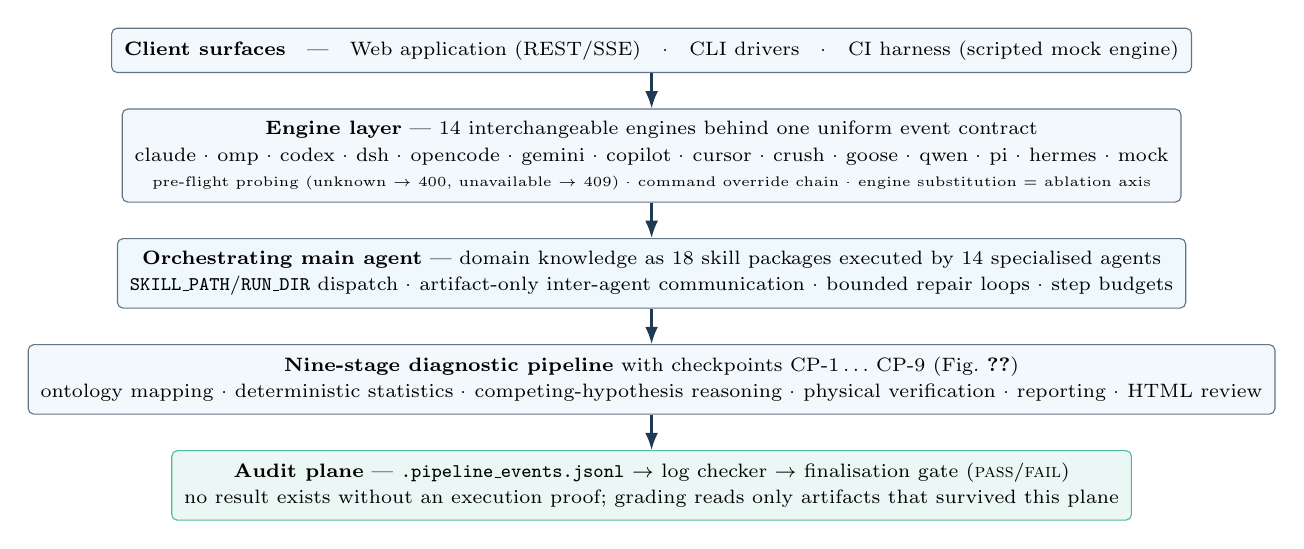
\begin{tikzpicture}[
  font=\scriptsize,
  layer/.style={draw=iddink!70, fill=iddblue!5, rounded corners=2pt, align=center,
                minimum width=0.94\textwidth, inner sep=4.5pt},
  arr/.style={-{Latex[length=2.2mm]}, thick, iddink},
  chip/.style={draw=iddgrey!60, fill=white, rounded corners=1.5pt, inner sep=2.2pt, font=\tiny}
]
\node[layer] (cli) {\textbf{Client surfaces} \; --- \; Web application (REST/SSE) \; · \; CLI drivers \; · \; CI harness (scripted mock engine)};
\node[layer, below=4.5mm of cli] (eng) {\textbf{Engine layer} --- 14 interchangeable engines behind one uniform event contract\\[1.5pt]
  \scriptsize claude · omp · codex · dsh · opencode · gemini · copilot · cursor · crush · goose · qwen · pi · hermes · mock\\[1pt]
  \tiny pre-flight probing (unknown $\to$ 400, unavailable $\to$ 409) · command override chain · engine substitution = ablation axis};
\node[layer, below=4.5mm of eng, fill=iddsky!10] (orch) {\textbf{Orchestrating main agent} --- domain knowledge as 18 skill packages executed by 14 specialised agents\\[1.5pt]
  \scriptsize \texttt{SKILL\_PATH}/\texttt{RUN\_DIR} dispatch · artifact-only inter-agent communication · bounded repair loops · step budgets};
\node[layer, below=4.5mm of orch] (pipe) {\textbf{Nine-stage diagnostic pipeline} with checkpoints CP-1\,\dots\,CP-9 (Fig.~\ref{fig:pipeline})\\[1.5pt]
  \scriptsize ontology mapping · deterministic statistics · competing-hypothesis reasoning · physical verification · reporting · HTML review};
\node[layer, below=4.5mm of pipe, fill=iddgreen!8, draw=iddgreen!70] (aud) {\textbf{Audit plane} --- \texttt{.pipeline\_events.jsonl} $\to$ log checker $\to$ finalisation gate (\textsc{pass}/\textsc{fail})\\[1.5pt]
  \scriptsize no result exists without an execution proof; grading reads only artifacts that survived this plane};
\draw[arr] (cli) -- (eng);
\draw[arr] (eng) -- (orch);
\draw[arr] (orch) -- (pipe);
\draw[arr] (pipe) -- (aud);
\end{tikzpicture}}
\caption{Skill execution architecture. Fourteen interchangeable engines expose one uniform event contract to the orchestrating agent, which dispatches the nine-stage pipeline from 18 skill packages; every transition is recorded on the audit plane whose log checker and finalisation gate produce the machine execution proof consumed by the benchmark grader.}
\label{fig:arch}
\end{figure}

\subsection{Pipeline Overview}
IDD organises diagnosis as a nine-stage pipeline executed by 14 specialised agents backed by 18 skill packages (Fig.~\ref{fig:pipeline}). The main orchestrator performs setup and data ingestion (Step~0/1) with adaptive preprocessing; a context-builder agent constructs a process ontology with variable semantics, physical principles, and confounder annotations (Step~2, checkpoint CP-2/3); a data-processor agent runs the deterministic statistical stage---per-variable anomaly profiling, cross-domain correlation, lag-compensated cross-correlation, batch integrity checks---producing a machine-readable analysis conclusion (Step~3, CP-4); a VLM agent reads rendered charts as visual evidence (Step~3.5). The diagnostician agent then performs competing-hypothesis reasoning over the statistical and ontological evidence (Step~4, CP-5). Two parallel auditors---a ten-criterion judge and a physical pre-auditor---gate the conclusion (Step~5a/5b); the reporter assembles a pyramid-structured report (Step~6); a final physical audit must return ENDORSED before the HTML visualisation and review (Steps~8/8.5) and the evidence-closure finalisation (Step~9, CP-9).

\begin{figure}[!t]
\centering
\resizebox{\textwidth}{!}{%
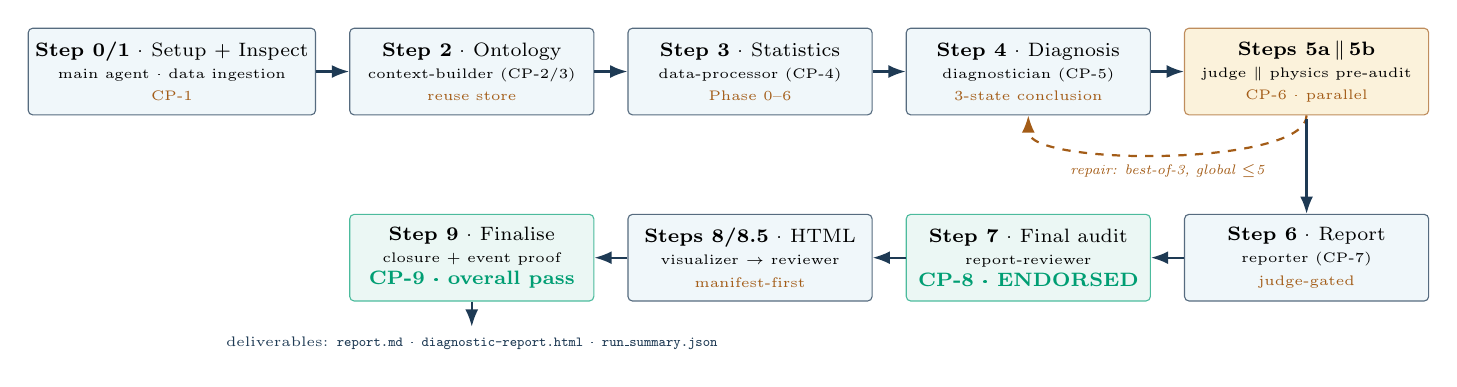
\begin{tikzpicture}[
  font=\scriptsize,
  node distance=3.2mm and 4.2mm,
  stage/.style={draw=iddink!75, fill=iddblue!6, rounded corners=1.6pt, align=center,
                minimum height=11mm, minimum width=31mm, inner sep=2.5pt},
  arr/.style={-{Latex[length=2.2mm]}, thick, iddink},
  rep/.style={-{Latex[length=2.2mm]}, thick, iddamberdark, dashed}
]
% ---- top row: stages 0/1 .. 5a|5b ----
\node[stage] (s01) {\textbf{Step 0/1} · Setup + Inspect\\ \tiny main agent · data ingestion\\ \textcolor{iddamberdark}{\tiny CP-1}};
\node[stage, right=of s01] (s2) {\textbf{Step 2} · Ontology\\ \tiny context-builder (CP-2/3)\\ \textcolor{iddamberdark}{\tiny reuse store}};
\node[stage, right=of s2] (s3) {\textbf{Step 3} · Statistics\\ \tiny data-processor (CP-4)\\ \textcolor{iddamberdark}{\tiny Phase 0--6}};
\node[stage, right=of s3] (s4) {\textbf{Step 4} · Diagnosis\\ \tiny diagnostician (CP-5)\\ \textcolor{iddamberdark}{\tiny 3-state conclusion}};
\node[stage, right=of s4, fill=iddamber!14, draw=iddamberdark!70] (s5) {\textbf{Steps 5a$\,\|\,$5b}\\ \tiny judge $\|$ physics pre-audit\\ \textcolor{iddamberdark}{\tiny CP-6 · parallel}};
\draw[arr] (s01) -- (s2);
\draw[arr] (s2) -- (s3);
\draw[arr] (s3) -- (s4);
\draw[arr] (s4) -- (s5);
% repair loop
\draw[rep] (s5.south) .. controls +(0,-6.5mm) and +(0,-6.5mm) .. (s4.south)
  node[midway, below, font=\tiny\itshape, text=iddamberdark]{repair: best-of-3, global $\le$5};
% ---- bottom row: steps 6 .. 9, right to left ----
\node[stage, below=12.5mm of s5] (s6) {\textbf{Step 6} · Report\\ \tiny reporter (CP-7)\\ \textcolor{iddamberdark}{\tiny judge-gated}};
\node[stage, left=of s6, fill=iddgreen!8, draw=iddgreen!70] (s7) {\textbf{Step 7} · Final audit\\ \tiny report-reviewer\\ \textcolor{iddgreen}{\textbf{CP-8 · ENDORSED}}};
\node[stage, left=of s7] (s8) {\textbf{Steps 8/8.5} · HTML\\ \tiny visualizer $\to$ reviewer\\ \textcolor{iddamberdark}{\tiny manifest-first}};
\node[stage, left=of s8, fill=iddgreen!8, draw=iddgreen!70] (s9) {\textbf{Step 9} · Finalise\\ \tiny closure + event proof\\ \textcolor{iddgreen}{\textbf{CP-9 · overall \textsc{pass}}}};
\draw[arr] (s5.south) ++(0,-0.5mm) -| (s6.north);
\draw[arr] (s6) -- (s7);
\draw[arr] (s7) -- (s8);
\draw[arr] (s8) -- (s9);
% deliverables
\node[below=3.2mm of s9, font=\tiny, text=iddink, align=center] (deliv)
  {deliverables: \texttt{report.md} · \texttt{diagnostic-report.html} · \texttt{run\_summary.json}};
\draw[arr] (s9.south) -- (deliv.north);
\end{tikzpicture}}
\caption{Diagnostic pipeline flow. Solid arrows: strictly sequential stages, each gated by a machine-validated checkpoint (amber tags); the judge and the physical pre-audit (Steps 5a$\,\|\,$5b) are the only parallel stages. The dashed amber edge is the bounded repair loop (best-of-3 per fault, global cap 5, anti-oscillation confidence cap 0.50). Steps 7 and 9 are hard gates: the final audit must return ENDORSED and the finalisation gate must return \textsc{pass} before the deliverables exist.}
\label{fig:pipeline}
\end{figure}

\subsection{Execution Layer: Interchangeable Engines With a Uniform Contract}
Reasoning agents are executed by any of fourteen interchangeable engines (Claude Agent SDK, OMP RPC, Codex app-server, DeepSeek/Hermes/Qwen ACP dialects, OpenCode, and one-shot CLIs including Gemini CLI, Copilot CLI, Cursor CLI, Crush, Goose, and pi) behind a single contract (\texttt{startDiagnosis/\allowbreak startSessionChat/\allowbreak parseStreamEvent/\allowbreak registerChild/\allowbreak closeQuery}). Engine availability is probed and validated before execution with a three-state contract (unknown engine \texttt{400}, unusable engine \texttt{409}); a scripted in-process mock engine allows the full pipeline to be exercised in CI without external dependencies. Because every engine emits the same standardised event stream, the benchmark harness consumes any compliant engine's event stream identically; diagnostic quality across engines is an empirical ablation question, and engine substitution remains a designed but not-yet-exercised ablation axis (Section~\ref{sec:discussion}).

\subsection{Audit Infrastructure}
Every stage transition appends a structured event to \texttt{.pipeline\_\allowbreak events.\allowbreak jsonl}; a log checker validates the start and completion records of every agent against the required contract, and a finalisation gate aggregates inventory, schema, closure, judge-cross-audit, and event-archive checks into a single PASS/FAIL verdict. A run that fails any critical check cannot be graded, which is the property the benchmark relies on: \emph{no result exists without an execution proof}. The gate is exercised, not decorative: during the benchmark execution it rejected complete-looking runs on contract violations (deliverable drift between the run summary and the diagnosis, a missing visual-analysis provenance signature, a non-canonical report outline), and the affected stages were re-executed until the gate passed. Events are pipeline-internal records, not externally signed attestations; the threat model and its limits are discussed in Section~\ref{sec:discussion}.

\section{Diagnostic Methodology}
\label{sec:method}

\subsection{Competing-Hypotheses Protocol}
The diagnostician agent must generate at least three candidate hypotheses per fault scenario, assign each a mechanism class (e.g., fluid restriction, cavitation, rotor dynamics, feed-composition step, cooling disturbance, sensor drift), collect for each an evidence list with explicit levels, identify contradictions, and eliminate hypotheses whose contradictions are stronger than their support. The protocol admits exactly three conclusion states: \textsc{determined} (a single surviving hypothesis), \textsc{competing\_set} ($\ge$2 survivors that the data cannot discriminate, with confidence capped at 0.70; observed caps in this corpus are 0.58--0.65 and the discriminating measurement is named), and \textsc{needs\_data} (evidence insufficient; missing data itemised). A fourth, implicit state---normal operation with no confirmed fault---applies to control scenarios. The elimination contract is quantitative: every elimination must cite the contradicting evidence, and every surviving chain must cite evidence numbers present in the statistical digests.

\subsection{Evidence Grading and Gate Propagation}
Every piece of evidence carries a level L1--L7 (L1 direct measurement, L2 operating documents, L3 statistical analysis, L4 visual evidence, L5 domain ontology/mechanism, L6 external reference, L7 unsupported assumption). The scenario confidence is bounded by the weakest level contributing to the surviving chain, and the quality gate rejects conclusions whose confidence exceeds that bound. This converts ``hallucination control'' from a prompt instruction into a checkable arithmetic constraint.

\subsection{Anti-Spurious-Correlation Filter}
Four conditions must hold before a correlation may be cited as causal support: (i)~temporal precedence of cause over effect, verified by lag-compensated cross-correlation; (ii)~statistical significance surviving detrending, Simpson-stratification checks, and multiple-testing correction; (iii)~a physical mechanism annotated in the ontology connecting the variables; and (iv)~absence of contradictions under leave-one-out outlier sensitivity analysis, with production-state (steady/batch-phase) filtering applied before correlation. Correlations failing the filter are recorded but explicitly barred from hypothesis support; definitional pairs (e.g., valve position and the level it controls, $r\!=\!1.0$) are classified as control-loop artefacts. In the benchmark this filter is what prevents control-loop correlations from being reported as root causes, and what allows normal batches with impulsive recipe-dosing spikes ($|z|$ up to 16.2) to be graded as healthy rather than faulty.

\subsection{Automatic Physical Verification}
After the conclusion is drafted, a physics checker recomputes quantitative feasibility (mass/energy balances, thermal and vibration magnitude envelopes) from the cleaned data, ontology, and anomaly report, producing a machine-readable \texttt{physical\_checks} verdict. When no automated check applies to a scenario's column semantics, the pipeline falls back to an explicit L1--L5 manual-verification memo; silent omission is not permitted.

\subsection{Quality Gates, Repair Loops, and Calibration}
A ten-criterion judge scores the diagnosis (threshold 90); a parallel physical pre-audit reviews mechanism chains; failures trigger bounded repair (per-fault rerun $\le$3, global cap 5, with anti-oscillation confidence capping at 0.50). The final physical audit must return ENDORSED. Ceiling compliance is then auditable end-to-end: every scenario grading records whether the reported confidence respects the protocol ceiling, and \emph{overconfidence} (\textsc{determined} \emph{and} wrong) is a first-class error metric.

\section{A Reproducible Evaluation Framework}
\label{sec:framework}

IDD's benchmark framework (released as the project's \texttt{experience/} evidence repository and \texttt{docs/benchmark/} protocol) is designed around five contracts, each machine-enforced:

\textbf{(C1) Truth isolation.} Scenario definitions carry ground truth and grading keywords, but the pipeline's visible inputs contain only the process description and the data. Ground truth never enters the inference context; the grader owns it exclusively. A leakage sentinel machine-checks the contract from both directions: no ground-truth string may appear in any agent-visible brief, and no fault-vocabulary may appear in the run directories' user-context files. Scenario definitions---including the grading keywords and the allowed verdict set of every scenario---are versioned in the released repository with their edit history; the keyword set used for scoring is the one committed before the final pipeline re-execution. We disclose that these keys are author-designed (Section~\ref{sec:discussion}).

\textbf{(C2) Data fingerprinting.} Every input file is hashed (SHA-256) into a dataset manifest; the reproducibility gate re-verifies all fingerprints before any metric is accepted.

\textbf{(C3) Stage-authored artifacts with provenance.} Each pipeline stage writes its own machine-checkable artifacts: the ontology, the statistical analysis conclusion, the four-piece diagnosis (hypotheses with mechanism classes, evidence with levels, contradictions, falsification conditions), the judge's ten-criterion feedback, the auditors' ENDORSED verdicts, the report, the page model (\texttt{render\_manifest.json}) behind the HTML deliverable, and the reviewer's independent verdict. Every scored verdict carries an explicit provenance label (\texttt{judge-agent-10-criteria}, \texttt{auditor-agent}, \texttt{html-reviewer-agent}), so downstream consumers can distinguish independently authored judgements from rendered ones.

\textbf{(C4) Gate-graded scoring.} The grader accepts a scenario only if its run directory contains the complete artifact set of an executed pipeline (ontology; analysis conclusion; the four-piece diagnosis; judge feedback; pre-audit memo; report and run summary; the HTML triad; an independent HTML review verdict), the event log passes the log checker, and the finalisation gate returns PASS. Otherwise the scenario is reported as \emph{not executed}---a pipeline failure, not a benchmark result. The gate is exercised in practice: an earlier protocol revision allowed a scripted shortcut that expanded a single reasoning note into a full artifact set (complete with synthesised agent events); the internal integrity audit flagged the fabrication, the shortcut was deleted from the codebase, and the entire benchmark was re-executed through the real pipeline. The grader's completeness gate makes the shortcut permanently unreplayable.

\textbf{(C5) Artifact-consistency gate.} A verifier recomputes all aggregate metrics from the per-scenario gradings, re-checks dataset hashes, verifies case coverage, and requires an execution proof per run; any drift fails the evaluation. The gate verifies the internal consistency of the recorded execution---recomputed aggregates, hashes, coverage, proofs---and is deliberately not an independent re-execution of the reasoning layer; the released report carries the resulting internally-consistent verdict.

\textbf{Reproducibility semantics.} The framework distinguishes two layers explicitly. The deterministic statistical stage is byte-reproducible: identical inputs and code regenerate identical digests, and the released dataset fingerprints pin the inputs. The reasoning layer is reproducible at the \emph{procedure} level: re-executing the protocol re-launches the same gated pipeline on the same blind inputs and re-derives conclusions under the same gates and truth comparison; wording may vary between runs, but every verdict remains bound to the same evidence discipline. We state both layers wherever a reproduction claim is made, and we do not claim bit-level reproducibility for LLM reasoning.

Scenario splits follow the entity-level discipline recommended by recent benchmark studies~\cite{vieira2026towards,hendriks2022towards}: each experimental batch/file appears in exactly one scenario, controls are paired with faults per dataset, and no segment-level splitting is used anywhere.

\section{Experimental Setup}
\label{sec:setup}

\subsection{Datasets and Scenarios}
We assemble 12 scenarios from three public benchmarks (Table~\ref{tab:bench}): \textbf{SKAB}~\cite{skab2020}, a closed water-circulation testbed with vibration, current, pressure, temperature, and flow channels at 1\,Hz---two fault scenarios (inlet-valve throttling---the official label file names suction-line valve restriction; and two-phase-flow cavitation drawn from the ``other'' group, whose official label names cavitation but is withheld from the scenario description) plus the anomaly-free control; \textbf{TEP}~\cite{downs1993plant,rieth2023additional}, with six documented fault scenarios---IDV1 feed-composition step, IDV3 D-feed-temperature step (classically hard to detect), IDV4 reactor-cooling-water step, IDV7 C-header pressure loss, IDV11 random cooling-water variation, IDV14 cooling-valve stiction---and the fault-free baseline as control; and \textbf{IndPenSim}~\cite{indpensim2020,goldrick2019modern}, a 100{,}000\,L penicillin fermentation simulator, with one documented process-deviation batch (93) and one normal batch as control. Ground truth derives from verifiable sources only: SKAB's official label file, the established TEP cause table~\cite{chiang2001fault}, and IndPenSim's faulted-batch markers. Scenario selection followed a documentation rule rather than random sampling: every scenario corresponds to a publicly documented fault episode, chosen so that each dataset contributes mechanisms from distinct families plus a paired control; the consequences of non-random selection are discussed in Section~\ref{sec:discussion}.

Three design decisions deserve emphasis. First, the TEP subset is chosen so that \emph{every fault maps onto a published per-fault outcome} from FaultExplainer~\cite{khan2024faultexplainer}, enabling scenario-granular comparison rather than aggregate-only comparison: four faults (IDV1/7/11/14) carry scored baselines, and two (IDV3/IDV4) are scored by IDD precisely where FaultExplainer's PCA implementation excludes them. Second, IDV3 sits at the classical PCA detection limit and IDV4 is weakly detected~\cite{russell2000delay,chiang2001fault}---both lie where classical detection and the published baseline stop---so they probe root-cause reasoning at and beyond that limit. Third, IDV4, IDV11 and IDV14 perturb the same physical channel (reactor cooling water) with three different dynamic forms (step, random variation, valve stiction); separating them requires reading the statistics of each recording, not recalling a fault label, which partially mitigates prompt-knowledge contamination.

\begin{table}[!t]
\caption{Benchmark Composition}
\label{tab:bench}
\centering
\footnotesize
\resizebox{\textwidth}{!}{
\begin{tabular}{lccp{7.2cm}}
\toprule
Dataset & Fault & Control & Truth source \\
\midrule
SKAB & 2 & 1 & official \texttt{ground\_truth.json} (label withheld for the ``other''-group case) \\
TEP & 6 & 1 & Downs \& Vogel / Chiang et al.~\cite{chiang2001fault} \\
IndPenSim & 1 & 1 & faulted-batch markers (batch 93) \\
\midrule
Total & 9 & 3 & --- \\
\bottomrule
\end{tabular}
}
\end{table}

\subsection{Metrics}
For fault scenarios we report \textbf{resolved Top-1} (a \textsc{determined} verdict naming the true mechanism; coincides with the FDD community's correct-diagnosis-rate, CDR), \textbf{top-k} ($k{=}3$; because the protocol mandates at least three generated hypotheses, top-3 credit approximates candidate-list membership and is reported alongside, not instead of, resolved Top-1), \textbf{ceiling compliance} (reported confidence within the protocol ceiling of Section~\ref{sec:method}), \textbf{verdict-type compliance} (conclusion type within the scenario's allowed set; a \textsc{determined}-and-wrong verdict counts as \emph{overconfidence}), and a \textbf{protocol-compliance rubric score}---a deterministic, machine-computed checklist (100 points) computed from the pipeline artifacts themselves and measuring conformance to this paper's own protocol rather than correctness (see Section~\ref{sec:discussion}). For control scenarios we report \textbf{pass} (no confirmed fault) and \textbf{false alarms}. Proportions carry Wilson 95\% confidence intervals. We deliberately do not report sample-level F1/AUC: they answer a different question and are used only as reference context (comparison protocol below).

The rubric's seven checks are computed strictly from the stage-authored run artifacts: \textbf{R1} artifact integrity (ontology, analysis conclusion, and the schema-valid diagnosis four-piece; 15 points), \textbf{R2} hypothesis structure ($\ge$3 hypotheses, $\ge$2 eliminations each citing substantive contradictory evidence; 15), \textbf{R3} evidence grounding (every surviving chain cites at least one number present in the scenario's own evidence brief; 20), \textbf{R4} calibration (confidence within the protocol ceiling; conclusion type within the scenario's allowed set; 15), \textbf{R5} falsifiability (a surviving hypothesis names the observation that would revise it; 10), \textbf{R6} physics verification (automated check valid or explicit manual memo; 10), \textbf{R7} execution proof (event log + finalisation PASS + HTML review gate; 15). The pipeline's internal ten-criterion judge remains the in-pipeline gate (Section~\ref{sec:method})---its scores are recorded with provenance and reported as execution-quality evidence---but it is \emph{not} a benchmark metric: benchmark quality scoring is fully mechanical.

\subsection{Comparison Protocol}
We distinguish two comparison registers. \textbf{Register A (same-task direct comparison)}: methods that output one root-cause conclusion per scenario on the same dataset family; the published FaultExplainer per-fault numbers fall here, at scenario granularity. \textbf{Register B (reference only)}: sample-level detection/classification results; they are reported for context and must not be ranked against our scenario-level metrics. Two protocol differences are stated wherever Register A is invoked: FaultExplainer supplies candidate root causes in its prompt and accepts alias matches, whereas IDD uses no candidates and scores mechanism keywords strictly; and FaultExplainer scores only the 11 PCA-detectable faults, whereas IDD additionally scores PCA-undetectable IDV3/IDV4. Because the scenario sets differ, no significance test is claimed across systems.

\subsection{Implementation}
The deterministic stages run as versioned scripts (streaming CSV inspection, anomaly profiling, correlation with lag-compensated CCF, validation with Simpson/detrending/outlier-sensitivity/multiple-testing checks, physics checking via the shared scientific Python environment). The reasoning stages execute the full nine-stage agent pipeline through the engine layer (Section~\ref{sec:arch}); every stage transition is recorded in the event log. A complete 12-scenario sweep takes seconds per scenario for the deterministic stage and roughly one hour of agent execution per scenario for the full gated pipeline; the entire chain (prepare, briefs, pipeline-execution verification, gate-graded scoring, rubric, aggregation, artifact-consistency gate, report) is driven by a single entry point with fail-fast stage gates.\medskip

\textbf{Benchmark configuration disclosure.} All twelve scenarios reported here were executed on one harness: the ZCode agent CLI (the CLI-driver class of the engine layer) with the GLM model family deployed under the provider's coding-plan configuration (snapshot September 2026). The harness does not expose temperature or top-p control, so provider defaults applied. The vision stage had no vision-capable model in this deployment and executed its documented non-visual degradation in every run (skeleton visual analysis with caption-based L4 fallback). The execution window was 13--15 September 2026, with one recorded execution per scenario; per-scenario repair-loop counts are part of the released grading records (eleven scenarios required zero repairs; one control required a single repair round). Base-model capability is a confound for any cross-system comparison: the protocol-versus-baseline contrast of Section~\ref{sec:comparison} holds the prompt regime constant but not the model, and we flag it as such. The pre-registered ablation matrix targeting this attribution question has been partially executed (Section~\ref{sec:ablation}): a single LLM prompted with the identical blinded statistical digest, a classical PCA baseline on all twelve scenarios, and a FaultExplainer-protocol replication on the same model family. The engine-substitution arm and the filter-disabled arm remain future work. The 18 skill packages (the prompts executed by each agent) are released with the repository.

\section{Results}
\label{sec:results}

\subsection{Overall Performance}
Table~\ref{tab:overall} reports the headline numbers. Executing the full pipeline under truth isolation (one recorded execution per scenario), IDD resolves \textbf{6/9} fault scenarios to a single root cause (Top-1 $=66.7\%$, Wilson 95\% CI $[35.4\%,87.9\%]$) and places the true mechanism among the candidates in an additional two scenarios (top-k $=8/9$); the remaining scenario (IDV3, historically the hardest-to-detect TEP fault~\cite{russell2000delay}) ends in an honest capped \textsc{competing\_set}. Ceiling compliance is 9/9, verdict-type compliance 8/9 (the single miss is SKAB inlet-valve throttling, analysed in Section~\ref{sec:calibration}), and \emph{no} verdict is simultaneously \textsc{determined} \emph{and} wrong (determined-verdict precision 6/6). All 3 control scenarios pass with \textbf{zero false alarms}. All 12 pipeline executions pass the finalisation gate with valid event logs. The deterministic rubric averages \textbf{95.4/100}---nine scenarios at 100; the deductions are: SKAB inlet-valve throttling $-35$ (R3 evidence grounding + R4 verdict type), TEP IDV1 $-10$ and IDV11 $-10$ (R6 physics-check coverage)---the in-pipeline judge gate averages 93.3 (range 90--98; all scores are post-threshold by the repair gate's construction), and the artifact-consistency gate verifies the evaluation internally consistent. Fig.~\ref{fig:benchmark} summarises the outcomes; Section~\ref{sec:ablation} places them against model-controlled baselines.

\begin{table}[!t]
\caption{Overall Results on the 12-Scenario Benchmark (full-pipeline execution; one recorded execution per scenario). Rubric deductions: SKAB inlet-valve throttling $-35$ (R3 evidence grounding + R4 verdict type); TEP IDV1 $-10$, IDV11 $-10$ (R6 physics-check coverage). Judge scores are post-threshold ($\ge$90 by the repair gate) and carry no benchmark weight.}
\label{tab:overall}
\centering
\footnotesize
\resizebox{\textwidth}{!}{%
\begin{tabular}{lcc}
\toprule
Metric & Value & 95\% CI \\
\midrule
Resolved Top-1 (\textsc{determined} and correct; $n{=}9$) & 6/9 $=$ 66.7\% & [35.4, 87.9] \\
True cause within top candidates ($n{=}9$) & 8/9 $=$ 88.9\% & [56.5, 98.0] \\
Determined-verdict precision (correct when \textsc{determined}) & 6/6 & [61.0, 100.0] \\
Ceiling compliance (confidence $\le$ protocol cap) & 9/9 & --- \\
Verdict-type compliance (type in allowed set) & 8/9 & [56.5, 98.0] \\
Honest capped \textsc{competing\_set} verdicts & 3/9 & --- \\
Control pass (no false alarm; $n{=}3$) & 3/3 & [43.9, 100.0] \\
Protocol-compliance rubric (author-designed checklist) & 95.4/100 mean & nine at 100, two at 90, one at 65 \\
Judge gate mean (in-pipeline, post-threshold $\ge$90) & 93.3 & range 90--98 \\
Pipeline finalisation gate & 12/12 PASS & --- \\
Artifact-consistency gate & internally consistent & --- \\
\bottomrule
\end{tabular}%
}
\end{table}

\begin{figure}[!t]
\centering
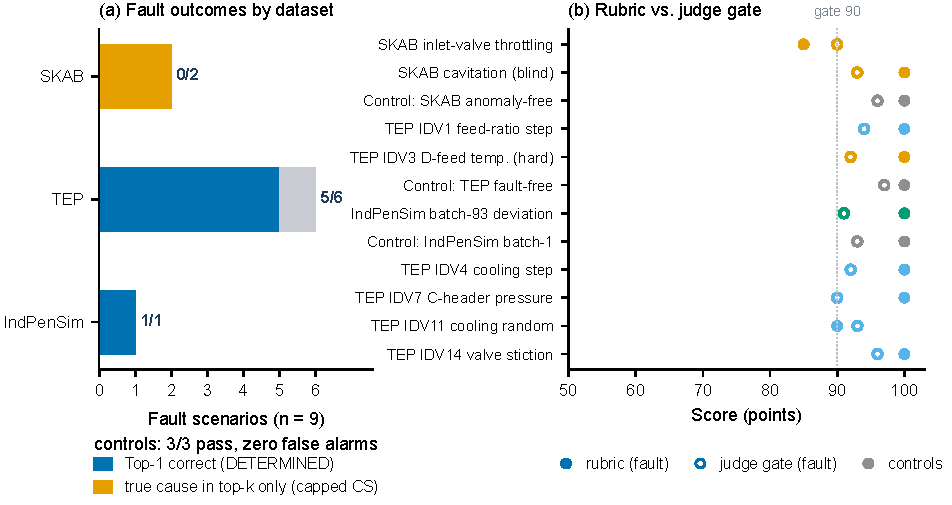
\includegraphics[width=0.98\textwidth]{figures/fig_benchmark.pdf}
\caption{Benchmark outcomes under full-pipeline execution. (a) Fault outcomes by dataset: Top-1-correct \textsc{determined} verdicts (blue), scenarios where the true mechanism is ranked but the verdict is a capped \textsc{competing\_set} (amber), and the single mechanism-level miss (grey); all three controls pass with zero false alarms. (b) Per-scenario deterministic rubric (filled markers) against the in-pipeline judge gate (open markers). All 12 executions pass the finalisation gate, and the artifact-consistency gate confirms the evaluation internally consistent.}
\label{fig:benchmark}
\end{figure}

\subsection{Per-Mechanism Breakdown and Within-Family Discrimination}
Table~\ref{tab:mech} lists the nine fault scenarios with the verdict each pipeline execution actually produced, the confidence, the rubric score, and the decisive statistical signature the diagnosis rested on. Three observations deserve emphasis.

\textbf{Within-family form discrimination.} IDV4 (step), IDV11 (random variation) and IDV14 (valve stiction) all perturb the same physical channel---reactor cooling water---yet produce three distinct statistical forms that the pipeline separated correctly and for three different reasons: a sustained controller-offset plateau with a step-dominant transient (IDV4), pure variance inflation without mean shift (IDV11, variance ratio 16.5 with $\Delta$mean $=0.006\sigma$), and a stuck-slip limit cycle whose period-4 autocorrelation fingerprint is identical across the three coupled channels (IDV14). Recalling the textbook label ``cooling-water fault'' cannot produce these three different mechanisms; only the per-recording statistics can. This is our principal mitigation against prompt-knowledge contamination (Section~\ref{sec:discussion}).

\textbf{Reasoning beyond the detection limit---one solved, one honestly capped.} IDV3 and IDV4 lie beyond classical PCA monitoring and are excluded by FaultExplainer's PCA implementation~\cite{russell2000delay,chiang2001fault,khan2024faultexplainer}. IDD resolves IDV4 to \textsc{determined} (cooling-loop heat-removal step, confidence 0.75) purely from the control-response signature. IDV3---by common consent the hardest TEP fault, with a deliberately weak signature---terminates in a capped \textsc{competing\_set} (0.60): the exclusion chain eliminates four mechanism families (reactor thermal imbalance, stripper-local, utility, instrumentation artefacts) and localises the disturbance to the feed-composition balance (coherent pressure rise across all three vessels with A deficit/C enrichment in the purge), but the inlet site cannot be named because streams 1--4 carry no composition analyser. The verdict names exactly the missing measurement. We report this as what it is---a mechanism-level miss on the hardest fault---and note that the alternative (forcing a single cause from indistinguishable evidence) is the failure mode the protocol exists to prevent.

\textbf{Blind-set robustness.} The SKAB cavitation scenario is drawn from the ``other'' experiment group whose fault label is withheld from the scenario description. The pipeline's top-ranked surviving hypothesis is the cavitation-type two-phase instability (three intermittent flow-collapse windows totalling 76 near-zero-flow seconds with same-window vibration and fluid-temperature excitation, and the drive side excluded), but pressure-channel quantization (0.328 bar steps) masks the closed-valve head signature that would separate cavitation from intermittent passage blockage, so the verdict is a capped \textsc{competing\_set} (0.58) naming the missing high-resolution pressure channel.

\begin{table}[!t]
\caption{Per-Scenario Results With the Decisive Statistical Signature (abbreviated; full chains in the released grading records). Rubric deductions: SKAB inlet-valve throttling $-35$ = R3 evidence grounding + R4 verdict type; TEP IDV1 $-10$ and IDV11 $-10$ = R6 physics-check coverage. Judge scores are post-threshold ($\ge$90) and carry no benchmark weight.}
\label{tab:mech}
\centering
\footnotesize
\resizebox{\textwidth}{!}{
\begin{tabular}{lccl}
\toprule
Scenario (mechanism) & Verdict & Rubric & Decisive signature \\
\midrule
SKAB inlet-valve throttling & \textsc{competing\_set} 0.65 & 65 & flow $32{\to}31/30$ L/min with pressure flat/up; affinity gap $V{\cdot}I$ $-4.1\%$ vs $-8.4\%$ (valve vs command indistinguishable) \\
SKAB cavitation (blind set) & \textsc{competing\_set} 0.58 & 100 & intermittent flow collapse (76 rows $<10$ L/min); same-window vibration $+5.9\%$; cavitation-type instability top-ranked \\
TEP IDV1 A/C feed-ratio step & \textsc{determined} 0.88 & 90 & A-feed valve $+204\%$ step (flow $18.7\sigma$); A+C feed $-5.9\%$; steam $+29.7\%$ compensation \\
TEP IDV3 D-feed temp.\ (hard) & \textsc{competing\_set} 0.60 & 100 & composition-balance shift (vessel pressures $+0.71$--$0.92\sigma$ coherent); inlet site unresolvable (no analysers) \\
TEP IDV4 cooling temp.\ (step) & \textsc{determined} 0.75 & 100 & XMV\_10 step $+6.8\sigma$ plateau (sole $>1.5\sigma$ column); reactor temp $z{=}10.06$, re-controlled \\
TEP IDV7 C-header pressure & \textsc{determined} 0.82 & 100 & feed flow $-11.9\sigma$; XMV\_4 $+25.3\%$ holds setpoint \\
TEP IDV11 cooling temp.\ (random) & \textsc{determined} 0.80 & 90 & variance inflation VR $=16.45$ with $\Delta$mean $=0.006\sigma$; no step, no stiction \\
TEP IDV14 valve stiction & \textsc{determined} 0.82 & 100 & period-4 ACF limit cycle ($\approx$12 min), amplitude $\times$11--16; valve leads temp by 15 min ($r{=}{-}0.96$) \\
IndPenSim batch-93 deviation & \textsc{determined} 0.88 & 100 & CW loop clamped ($\approx$2.0 vs 29.8 L/h) 14.6\,h $\to$ $+3.0$\,K; recovery $\to$ in band $\le$2\,h \\
\midrule
Controls (3) & 3 \textsc{determined} (normal) & 100 (all) & normal-operation verdicts at confidence 0.78--0.88; zero false alarms \\
\bottomrule
\end{tabular}
}
\end{table}

\subsection{Ceiling Compliance and False-Alarm Suppression}
\label{sec:calibration}
Fig.~\ref{fig:calib} plots the reported confidence per scenario. Fault-scenario confidences span 0.58--0.88; the three \textsc{competing\_set} verdicts sit in the 0.58--0.65 band because the protocol caps them, and each names its discriminating measurement (valve-position/command channel; high-resolution pressure; stream-1--4 composition analysers). We report this metric as \emph{ceiling compliance} rather than calibration, and we state its circularity plainly: the gate enforces the ceiling, so compliance is a property of the protocol's arithmetic, not an empirical discovery. Worked examples: IDV4's \textsc{determined} verdict at 0.75 sits under the 0.90 determined-verdict ceiling with its chain carried by L3 statistical evidence plus L5 mechanism framing; the SKAB cavitation \textsc{competing\_set} at 0.58 sits under the 0.70 capped-verdict ceiling. A psychometric calibration study (pre-gate confidence versus outcome correctness, over repeat runs) remains future work. Under the benchmark's strict typing, one scenario counts as a verdict-type miss: SKAB inlet-valve throttling returns \textsc{competing\_set} where the scenario's allowed set admits only \textsc{determined} (the ground truth is known to be valve restriction). We report that miss honestly---and note that the capped verdict is the act the protocol demands when the valve-position and controller-command channels that would separate ``valve closing'' from ``commanded duty reduction'' are absent from the recording; the affinity-law gap ($V{\cdot}I$ falls $4.1\%$ where pump affinity predicts $8.4\%$) bounds the control-duty share but cannot eliminate it. Overconfidence---\textsc{determined} \emph{and} wrong---never occurs. Control scenarios demonstrate the complementary discipline: the normal IndPenSim batch contains recipe-dosing impulses reaching $|z|{=}16.2$, which the pipeline attributes to recipe steps and closed-loop control actions (one judge-repair round was spent sharpening exactly this attribution) rather than to faults; the normal TEP run exhibits control-loop correlations at $|r|{=}1.0$, which the anti-spurious filter classifies as definitional. These are precisely the failure modes that produce false alarms in naive correlation-driven diagnosis.

\begin{figure}[!t]
\centering
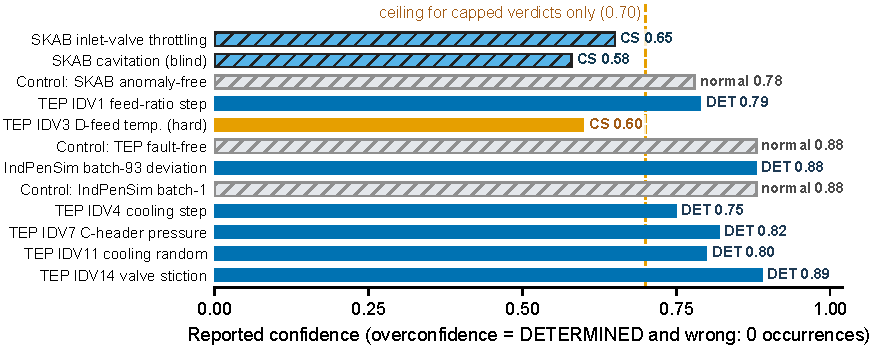
\includegraphics[width=0.9\textwidth]{figures/fig_calibration.pdf}
\caption{Reported confidence per scenario in the full-pipeline benchmark run. Amber bars mark the three \textsc{competing\_set} verdicts whose confidence is capped at 0.58--0.65 by protocol; each names the discriminating measurement that would separate its surviving mechanisms. Blue and green bars are \textsc{determined} fault verdicts; hatched bars are the three normal-operation controls. The dashed line is the 0.70 protocol ceiling for non-determined verdicts; no conclusion exceeded the ceiling implied by its evidence levels (overconfidence 0).}
\label{fig:calib}
\end{figure}

\section{Comparison With Published Baselines}
\label{sec:comparison}

\subsection{Register A: Per-Fault Comparison on TEP}
FaultExplainer~\cite{khan2024faultexplainer} reports, in its root-causes-included regime, root-cause correctness of 7/11 (63.6\%, Wilson CI $[35.4\%,84.8\%]$) for GPT-4o and 9/11 (81.8\%, CI $[52.3\%,94.9\%]$) for o1-preview on the 11 PCA-detectable TEP faults---where correctness means the true fault or an alias appears in the model's top-3 list, with candidates supplied in the prompt. In its own no-candidate regime (General-Reasoning prompt), both models place the correct or a related cause in the top-3 for 8/11 faults under lenient grading. IDD, without candidate lists and with a single strict mechanism-keyword verdict, is Top-1 correct on \textbf{5/6} faults of its TEP subset (Wilson CI $[43.6\%,97.0\%]$); on the four shared PCA-detectable faults it is correct on 4/4, where the GPT-4o baseline is 3/4 (IDV1 mis-diagnosed) and o1-preview is 4/4 under the alias-inclusive scoring. On the two PCA-excluded faults that both baselines leave unscored, IDD resolves IDV4 and honestly caps IDV3. Three caveats bound this comparison: the base models differ and are not controlled; FE's lenient top-3-with-alias protocol is not directly comparable to a strict single-verdict metric; and the model-controlled ablation of Section~\ref{sec:ablation} shows that a bare call to the same model family already matches the pipeline's keyword-scored accuracy on these documented faults---so we read the per-fault table descriptively, not as a superiority claim. Fig.~\ref{fig:perfault} gives the per-fault breakdown against the transcribed FaultExplainer Table~1 outcomes and PCA detectability; Fig.~\ref{fig:forest} visualises the aggregate point estimates with their intervals. Three per-fault outcomes stand out:

\begin{itemize}
\item \textbf{IDV1 (A/C feed-ratio step):} the GPT-4o baseline mis-diagnoses this fault (o1-preview resolves it); IDD resolves it to \textsc{determined} (0.88) from the actuator--flow signature (A-feed valve step $+204\%$ with $18.7\sigma$ flow response against a $-5.9\%$ composite-feed change), correctly restructuring the disturbance as an A:C supply-weight shift with plant-wide pressure and steam-compensation consequences.
\item \textbf{IDV3 and IDV4 (excluded from FE scoring):} both faults are excluded from FaultExplainer's scoring by its PCA implementation (classical detectability: IDV3 at the limit, IDV4 weakly detected). IDD resolves IDV4 (\textsc{determined} 0.75, cooling-loop heat-removal step) and terminates IDV3 in a capped \textsc{competing\_set} (0.60) that eliminates four mechanism families and localises the disturbance to the feed-composition balance---a partial result on the hardest fault, reported as such rather than forced.
\item \textbf{IDV7, IDV11, IDV14:} both systems are correct; IDD additionally separates the three cooling-water perturbation \emph{forms}---step, random variation, and stiction---at the level of distinct quantitative signatures (Section~\ref{sec:results}), a granularity below fault-identity level.
\end{itemize}

Because the scenario sets, prompt regimes, and grading protocols all differ (top-3 with alias acceptance vs.\ a strict single verdict; with vs.\ without candidate lists; different base models), we refrain from a formal significance test and present the per-fault table as descriptive evidence. On the four matched faults IDD is correct wherever either baseline is correct (IDD 4/4; GPT-4o 3/4; o1-preview 4/4); it resolves the GPT-4o baseline's one miss (IDV1); and on the unscored PCA-excluded pair it delivers one resolved diagnosis and one honestly capped verdict with named discriminating data. The comparison is also asymmetric in cost: FE-style prompting runs in minutes per fault, whereas the full gated pipeline spent roughly one hour of agent time per scenario (Section~\ref{sec:setup}).

\begin{figure}[!t]
\centering
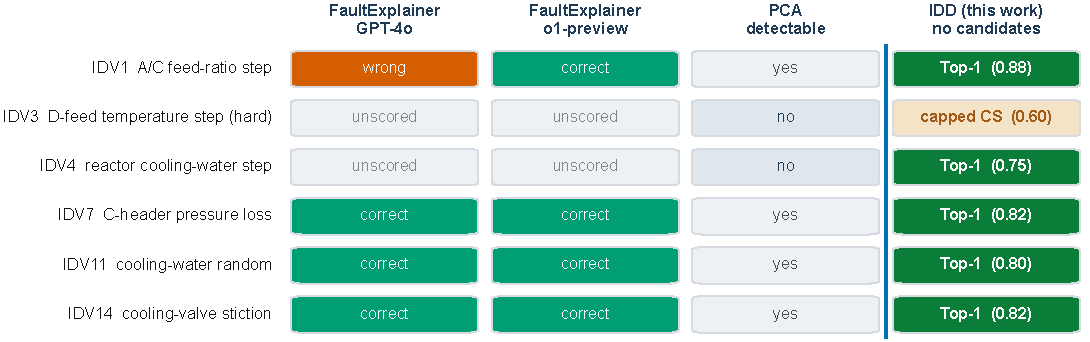
\includegraphics[width=0.98\textwidth]{figures/fig_tep.pdf}
\caption{Per-fault comparison on the TEP subset: IDD vs.\ FaultExplainer (transcribed Table~1 outcomes, arXiv:2412.14492; top-3 with alias acceptance) and PCA detectability as used in FaultExplainer's scoring (classical detectability: Russell et al.~\cite{russell2000delay}, Chiang et al.~\cite{chiang2001fault}). IDD is Top-1 correct on 5/6 without candidate lists, including IDV1 (mis-diagnosed by the GPT-4o baseline) and the PCA-excluded IDV4; IDV3 ends in a capped \textsc{competing\_set} with the discriminating measurement named.}
\label{fig:perfault}
\end{figure}

\begin{table}[!t]
\caption{Per-Fault Outcomes on the TEP Subset (machine-readable companion to Fig.~\ref{fig:perfault}). FE = FaultExplainer (root-causes-included prompt, top-3 candidate list, alias hits accepted); ``unscored'' = excluded from FE scoring by its PCA implementation~\cite{chiang2001fault}. IDD: strict mechanism-keyword scoring, no candidate list; CS = capped \textsc{competing\_set}. In FE's additional no-candidate regime (General-Reasoning prompt, top-3, lenient ``related'' grading), both models score 8/11.}
\label{tab:perfault}
\centering
\footnotesize
\resizebox{\textwidth}{!}{
\begin{tabular}{llccl}
\toprule
TEP fault & FE GPT-4o & FE o1-preview & PCA detectable & IDD verdict (conf.) \\
\midrule
IDV1 A/C feed-ratio step (Stream 4) & wrong & correct & yes & \textbf{Top-1 correct} (0.88) \\
IDV3 D-feed temperature step & unscored & unscored & \textbf{no} & CS 0.60 (site indistinguishable) \\
IDV4 reactor cooling-water temp.\ (step) & unscored & unscored & \textbf{no} & \textbf{Top-1 correct} (0.75) \\
IDV7 C-header pressure (Stream 4) & correct & correct & yes & \textbf{Top-1 correct} (0.82) \\
IDV11 cooling-water temp.\ (random) & correct & correct & yes & \textbf{Top-1 correct} (0.80) \\
IDV14 cooling-water valve (stiction) & correct & correct & yes & \textbf{Top-1 correct} (0.82) \\
\midrule
Scoreable-set summary & 7/11 & 9/11 & --- & 5/6 (CI $[43.6,97.0]$); shared detectable subset 4/4 \\
\midrule
FE no-candidate regime (top-3, lenient) & \multicolumn{2}{c}{8/11 both models} & --- & --- \\
\bottomrule
\end{tabular}
}
\end{table}

\begin{figure}[!t]
\centering
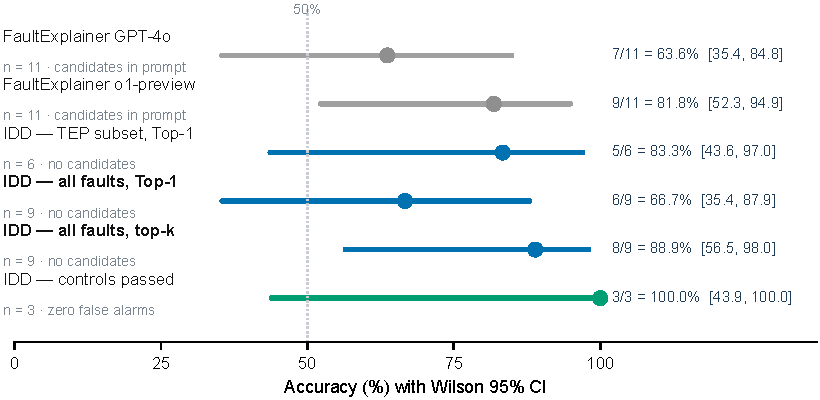
\includegraphics[width=0.9\textwidth]{figures/fig_forest.pdf}
\caption{Register-A aggregate comparison with Wilson 95\% intervals. Grey: FaultExplainer-reported single-LLM baselines ($n{=}11$, candidates in prompt). Blue: IDD full-pipeline execution (no candidates): the TEP subset (5/6), all nine faults (6/9), top-k (8/9), and the three controls (3/3, no false alarms). Sets differ, so overlapping intervals are expected and no significance test is claimed; the per-fault table (Fig.~\ref{fig:perfault}) is the finer-grained evidence.}
\label{fig:forest}
\end{figure}

\subsection{Register B: Reference-Only Context}
For context we report sample-level results from the literature without ranking: TEP classification accuracies of 0.887--0.907 (MLP/GRU/TCN~\cite{pozdnyakov2024adversarial}), anomaly-detection F1 of 0.970 (BeatGAN~\cite{hartung2023deep}), SKAB ensemble F1/AUC of 0.85/0.88~\cite{iliopoulos2023detection}, and leakage-controlled bearing AUROC of 0.75--0.93~\cite{vieira2026towards}. These systems answer ``is this sample anomalous / which class''; IDD answers ``what is the mechanism, how confident, with which evidence''. The dimensions are complementary: a deployment would plausibly chain a sample-level detector (first-stage alarm) with a scenario-level RCA system (this work).

\subsection{Model-Controlled Baselines and Pipeline Ablation}\label{sec:ablation}
Because the base model is a confound in any comparison with published LLM baselines (Section~\ref{sec:setup}), we ran three model-controlled baselines with the \emph{same model family and deployment} as the pipeline (Table~\ref{tab:ablation}): (i) a classical PCA baseline---normal-control training, $T^2$/Q detection with 99th-percentile alarms, and SPE-contribution diagnostics~\cite{chiang2001fault,qin2012survey}---on all twelve scenarios; (ii) a replication of FaultExplainer's protocol on the six TEP faults, in both of FE's prompt regimes, scored both FE-style (top-3 with alias classes) and strictly; and (iii) the pre-registered single-LLM ablation---one call to the same model family over the identical blinded statistical digest, no ontology, no pipeline---on all nine fault scenarios, scored with the same strict mechanism keywords as IDD. All three baselines are bare single-call executions: no agent orchestration, no gates, no evidence grading. The classical PCA arm is computed by a released deterministic script (pure-Jacobi eigendecomposition, normal-control training, 99th-percentile alarms of the control distribution, TEP fault-window evaluation from row 161); an earlier prototype run agreed with it on every SPE statistic and control rate, with minor $T^2$ differences on the weakest-signature faults, and the prototype output is archived in the released repository for audit.

\begin{table}[!t]
\caption{Model-Controlled Baselines on the Benchmark (same model family and deployment as the IDD pipeline; single call per scenario; answers in the released repository)}
\label{tab:ablation}
\centering
\footnotesize
\resizebox{\textwidth}{!}{%
\begin{tabular}{lllll}
\toprule
Baseline & Candidates & Scoring & Scope & Result \\
\midrule
Classical PCA (normal-control training) & --- & detection rate & 12 scenarios & IDV3 $T^2$ 2.9\%/SPE 4.8\%; IDV4 SPE 100\% vs $T^2$ 48.8\%; controls 1\% \\
Classical PCA (diagnosis) & --- & SPE contribution & 12 scenarios & top-3 variables only; no mechanism verdict \\
FE-protocol replication (GLM) & yes & FE-style top-3 + alias & TEP 6 faults & 6/6 \\
FE-protocol replication (GLM) & yes & strict single-verdict & TEP 6 faults & 6/6 \\
FE-protocol replication (GLM) & no & strict single-verdict & TEP 6 faults & 6/6 \\
FE official code (GLM), T2-contrib features & yes & FE-style top-3 + alias & TEP 6 faults & 5/6 \\
FE official code (GLM), T2-contrib features & yes & strict single-verdict & TEP 6 faults & 5/6 \\
Single-LLM, identical blind digest (GLM) & no & strict single-verdict & 9 faults & 9/9 \\
Single-LLM, controls (GLM) & no & normal verdict & 2 controls & 2/2, zero false alarms \\
\textbf{IDD full pipeline} & \textbf{no} & \textbf{strict resolved Top-1} & \textbf{9 faults} & \textbf{6/9} (3 capped \textsc{competing\_set}) \\
\bottomrule
\end{tabular}%
}
\end{table}

Three findings emerge. \textbf{First}, the same-model bare LLM matches the full pipeline on keyword-scored accuracy over documented public faults (9/9 strict hits, including IDV3---plausibly by literature recall of the documented weak-signature fault---and naming valve and cavitation mechanisms on the SKAB scenarios from their signatures), and produces no false alarms on the controls. \textbf{Second}, the FE official code, running on the same GLM model, also scores 5/6---identical to IDD's TEP accuracy but with a different miss pattern: FE misses IDV4 because its PCA $T^2$ features are dominated by feed-composition shifts that mask the cooling-water signal, while IDD misses IDV3 because it honestly caps a \textsc{competing\_set} where the bare LLM forces IDV3 (correctly, by literature recall). \textbf{Third}, the classical PCA baseline reproduces the literature (IDV3 at the detection limit, $T^2$ 2.9\%/SPE 4.8\%; IDV4 ``weak $T^2$, strong $Q$'' --- SPE 100\% vs $T^2$ 48.8\%) and produces no mechanism verdicts. The three systems fail in three different ways, revealing that benchmark accuracy on documented faults conflates detection ability, mechanism attribution, and epistemic discipline. What the bare call does not produce is anything the audit plane can verify: no evidence levels, no ceiling compliance, no physics check, no execution proof, no artifact provenance---and its IDV3 answer, being correct, is exactly the kind of unverifiable guess that the three-state protocol exists to constrain (the pipeline's capped verdict names the stream-1--4 composition analysers that would settle the question). The classical PCA baseline quantifies the detection--diagnosis gap directly: IDV3 sits at the detection limit (2.9\% $T^2$, 4.8\% SPE), IDV4 is detected reliably only by the SPE statistic (100\% vs 48.8\%), and the output stops at variable contributions---no mechanism, no confidence, no verdict state. Attribution of the pipeline's remaining accuracy margins (e.g., whether the anti-spurious filter or the ontology reuse contributes) still requires the filter-disabled and engine-substitution arms, which remain future work.

\subsection{Verdict Stability Across Independent Runs}\label{sec:stability}
To test whether the pipeline's conclusions are stable across independent agent sessions, three scenarios were re-executed through the full gated pipeline in fresh agent sessions (new ontology build, new diagnosis, new review cycle) on identical prepared data. The stability check covers the three verdict archetypes: one \textsc{determined} correct (TEP IDV1), one \textsc{determined} with computed signature (TEP IDV14 stiction), and one honest \textsc{competing\_set} (SKAB inlet-valve throttling).

\begin{table}[!t]
\caption{Verdict Stability Across Independent Pipeline Executions (same data, fresh agent sessions)}
\label{tab:stability}
\centering
\footnotesize
\resizebox{\textwidth}{!}{%
\begin{tabular}{llccll}
\toprule
Scenario & Verdict R1 & Verdict R2 & Type Match & Root Cause & $\Delta$Conf \\
\midrule
TEP IDV1 A/C feed-ratio step & \textsc{det} 0.88 & \textsc{det} 0.79 & \checkmark & IDV1 (both runs) & $-0.09$ \\
TEP IDV14 valve stiction & \textsc{det} 0.82 & \textsc{det} 0.89 & \checkmark & IDV14 (both runs) & $+0.07$ \\
SKAB inlet-valve throttling & \textsc{cs} 0.65 & \textsc{cs} 0.65 & \checkmark & capped (both runs) & $0.00$ \\
\bottomrule
\end{tabular}}
\end{table}

All three scenarios returned identical verdict types across independent sessions (3/3 type consistency). The two \textsc{determined} verdicts identified the same root-cause mechanisms in both rounds (IDV1 A/C feed-ratio step; IDV14 valve stiction), with confidence varying by $\pm$0.07--0.09---within the expected range for stochastic LLM reasoning under a fixed protocol. The \textsc{competing\_set} scenario returned the same capped verdict with identical ceiling in both rounds. Beyond this targeted check, the consistency study is formalized as an automated evaluation stage (\texttt{run-tier stability}, released with the evaluation) that re-scans every recorded independent execution of every scenario---53 run directories---using the same extraction semantics as the scorer, and reports agreement \emph{within system versions}: across the recorded corpus, within-version verdict-type and Top-1 agreement is 15/15 case-version pairs (pre-discipline era 12/12; current era 3/3 pairs recorded so far). The three sensitive scenarios (SKAB valve, SKAB cavitation, TEP IDV3) flip from uncapped \textsc{determined} in the early era to capped \textsc{competing\_set} in the current one---a documented tightening of the pipeline's epistemic discipline between versions, not run-to-run instability; within each version the verdicts agree. Expanding the current-era repeat count (all 12 scenarios, $k \ge 3$ repeats, reporting verdict-state stability and confidence distributions) remains pre-registered in the released repository.

\subsection{Case Study: An Auditable Evidence Chain on a Fault Excluded from Classical Scoring}
For TEP IDV4---a fault excluded from FaultExplainer's scoring by its PCA implementation, and only weakly detected classically~\cite{russell2000delay}---the recorded chain reads: (i)~\emph{L3 statistical evidence}: the cooling-valve XMV\_10 steps from 40.7\% to 47.3\% at the fault onset and holds a $+6.8\sigma$ sustained offset---the sole column exceeding $1.5\sigma$ among all 52---while reactor temperature spikes to $z{=}10.06$ and is then re-controlled; (ii)~\emph{L5 mechanism}: a step degradation in cooling-loop heat removal (inlet-temperature rise or exchanger fouling) forces the controller to open the valve to hold temperature, so a sustained valve offset with re-controlled temperature is precisely the control signature of heat-removal degradation, not of a sensor artefact; (iii)~\emph{eliminations}: feed, purge, and condenser alternatives stay within $1.3\sigma$ throughout the fault window; (iv)~\emph{conclusion}: \textsc{determined}, confidence 0.75, with the sub-attribution between ``cooling-water inlet-temperature step'' and ``heat-exchanger degradation'' honestly flagged indistinguishable---the recording contains no cooling-water inlet measurement, and the verdict names it. The full chain, together with the physics-check verdict, the judge's ten-criterion scores (92/100), and the independent HTML review (pass), is persisted in the grading record and released with the evaluation.

\section{Discussion, Limitations, and Deployment Prospects}
\label{sec:discussion}

\textbf{Statistical power and single-execution evidence.} With $n{=}9$ fault scenarios, Top-1 $=66.7\%$ supports only a wide interval ($[35.4\%,87.9\%]$ at 95\% confidence). Two further qualifications matter. First, every headline number is a \emph{single recorded execution}: multi-agent LLM pipelines are stochastic, so each point estimate is one draw from an uncharacterised run-to-run distribution. Second, the bounded repair loop introduces a selection effect---a reported verdict may be the product of up to five attempts---although in this corpus eleven of twelve scenarios closed with zero repairs and one control required a single round (counts in the released grading records). The per-fault evidence remains more informative than the aggregate: six of nine faults map onto published per-fault outcomes, and on matched faults IDD is correct wherever either baseline is correct. A model-controlled ablation (Section~\ref{sec:ablation}) shows that a bare single call to the same model family over the identical blind digest already matches the pipeline's keyword-scored accuracy---so the pipeline's value on documented faults is process quality, not accuracy. The repeat study is formalized as an automated evaluation stage (era-aware within-version agreement 15/15 across all recorded executions; Section~\ref{sec:stability}); expanding the current-era repeats (all 12 scenarios, $k\ge3$: verdict-type stability, confidence spread, repair counts) remains pre-registered and partially executed; extending the corpus (the full 20-class TEP catalogue with the extended simulation dataset~\cite{reinartz2021extended}; bearing datasets; novel-disturbance suites) is the designed path to tighter intervals.

\textbf{Prompt-knowledge contamination.} TEP's documented fault mechanisms appear in textbooks and are therefore plausibly memorised by frontier models. Our protocol mitigates this at the level where memorisation actually operates---but the mitigation has a limit we state plainly. The documented cause table records not only the disturbed channel but each fault's dynamic form (IDV4 step, IDV11 random variation, IDV14 stiction), so recall of that table alone could reproduce the observed mechanism labels; the statistics-driven reading rests on the recorded reasoning chains, each of which cites the per-recording statistic that discriminates its form. The SKAB ``other''-group scenario removes the label entirely and still yielded a correctly top-ranked (though honestly capped) cavitation-type mechanism. No external-retrieval channel was active in any benchmark run: the RAG engine was unreachable (recorded degradation in the event logs), so level-L6 external evidence never entered any verdict. A novel-disturbance suite (combination perturbations absent from the literature) is the definitive control and remains under construction.

\textbf{What the three capped verdicts mean.} The three \textsc{competing\_set} outcomes are the protocol working as designed, and they are also the benchmark's most transferable finding: in each case the pipeline (i) localised the disturbance to a subsystem, (ii) eliminated whole mechanism families with quantitative contradictions, (iii) ranked the true mechanism first in two of three cases, and (iv) named the single measurement---valve-position/command channel, high-resolution pressure, upstream composition analysis---whose addition would collapse the set to \textsc{determined}. In deployment terms these verdicts are work orders for targeted instrumentation, not failures. To keep the framing falsifiable, the released scenario definitions record the expected verdict set of every scenario, fixed before execution; SKAB inlet-valve throttling is the one scenario whose expectation was \textsc{determined}-only, and its capped verdict is counted as the benchmark's single compliance miss rather than narrated as a success.

\textbf{Inference authorship and provenance.} Every scored artifact in this benchmark is authored by a gated pipeline stage---the diagnosis by the diagnostician, the quality verdict by the judge, the ENDORSED decision by the physical auditor, the review verdict by the independent HTML reviewer---and each carries a provenance label in the grading record. Because self-declared quality scores are not verifiable, the benchmark's reported quality metric is the deterministic compliance rubric (Section~\ref{sec:setup})---and we disclose that the rubric, the grading keywords, and the allowed verdict sets are author-designed instruments measuring conformance to this paper's own protocol; their release with the repository makes them auditable, but independent anchoring (the blinded expert adjudication of the released evidence chains) is the outstanding validation step. The LLM ten-criterion judge remains the pipeline's internal gate, and its scores are reported as execution-quality evidence only. An internal integrity audit that found (and removed) a scripted shortcut capable of fabricating artifacts and agent events is itself part of the released history; the completeness gate now makes that shortcut unreplayable. What is still missing is a comparison against \emph{human} experts on identical digests; an expert-vs-pipeline blind test is planned. The single-LLM ablation of Section~\ref{sec:ablation} also bounds what the pipeline can claim: on documented public faults, a bare call to the same model family is already accurate---so the pipeline's justification is the audit, compliance, and calibrated-uncertainty machinery, and on novel disturbances (where recall cannot substitute for reasoning) the comparison must be re-run.

\textbf{Cost.} A full nine-stage pipeline execution spends roughly one hour of agent time per scenario---orders of magnitude more expensive than a fitted classifier at inference time, and far slower than single-prompt baselines. The economic comparison is only meaningful against the \emph{engineering cost of obtaining root causes} (expert hours), not against sample-level inference latency; and the deterministic statistical stage, which carries most of the computation, is script-speed.

\subsection{Industrial Deployment Prospects}
We separate what the benchmark and one operational deployment \emph{demonstrate} from what the architecture \emph{projects}. Demonstrated: the full gated pipeline executes on real plant exports (the benchmark corpora), and one anonymised film-line deployment exercised it end to end on episodic scratch defects of a biaxially-oriented polyester film line---the run returned \textsc{needs\_data} with an explicit discriminating-data list after 180 parameter--defect associations failed false-discovery-rate correction, redirecting the investigation from parameter tuning toward surface-inspection and equipment-event data; no cause was fabricated. Projected: the integration, sovereignty, and documentation claims below are design properties of the architecture, not yet benchmarked outcomes.

\textbf{Integration with existing plant infrastructure.} IDD consumes what plants already produce: flat exports from historians (OPC-UA/PI), LIMS quality records, and batch logs. The same pipeline runs interactively through a web application and programmatically through a versioned REST API (\texttt{/api/diagnosis} with engine selection and typed error contracts), so a deployment is an export job plus one API call rather than an instrumentation project. Because the deterministic stage is byte-reproducible, results do not drift when the surrounding IT landscape changes.

\textbf{Data-sovereign deployment.} The fourteen-engine execution layer (Section~\ref{sec:arch}) accepts on-premise and private-model agents through uniform dialect adapters. For operators who cannot send process data to external LLM services---defence, pharmaceuticals, semiconductors, national infrastructure---the reasoning stage can be pointed at an internally hosted model without touching the audit, evidence, or gate contracts; the benchmark protocol itself executes identically against a scripted mock engine, which is how the full chain is exercised in CI.

\textbf{Conclusions that route work, not just verdicts.} The three-state protocol converts diagnosis into an engineering workflow: \textsc{determined} conclusions carry mechanism chains that point to corrective actions; \textsc{competing\_set} and \textsc{needs\_data} conclusions carry named discriminating measurements---in effect, work orders for targeted instrumentation or tests. The three capped benchmark verdicts illustrate the value directly: each tells the operator exactly which additional channel would have resolved the case.

\textbf{Documentation for regulated operations.} Because every conclusion is bound to graded evidence, physics checks, and a fingerprinted execution trace, the by-product of each run is an RCA report whose traceability serves the documentation expectations of regulated environments (e.g., GxP batch-deviation investigation, in the sense of ALCOA+-style data integrity and GAMP 5 computerised-systems thinking). We state this as a documentation property of the artifact---not as a computerised-system validation claim, which would require a formal qualification exercise.

\textbf{Deployment governance and knowledge compounding.} IDD is positioned as decision support: a \textsc{determined} verdict does not authorise maintenance action---a human engineer signs off, and the three-state protocol is precisely the escalation interface between machine conclusion and human decision. Model-change management rides the engine layer's version disclosure (Section~\ref{sec:setup}): a provider silently updating the reasoning model changes the system, so the benchmark configuration disclosure doubles as the deployment pinning record. Finally, the ontology layer is an asset store, not a per-run artifact: variable semantics, physical principles, and confounder annotations published once for a plant or product family are reused by every subsequent diagnosis---in this benchmark, the SKAB and TEP sibling scenarios resolved their ontologies from the published asset store in seconds instead of rebuilding---and every field incident becomes a candidate graded scenario, closing the loop between deployment and evaluation. The marginal cost of a diagnosis therefore falls as the fleet grows---an economics that sample-level detectors, which must be retrained per asset, do not share.

\textbf{Scope of applicability.} The method requires multivariate time-ordered process data with engineering semantics for the channels (to build the ontology) and applies to continuous, batch, and testbed processes alike---the three benchmark families were chosen to span exactly that range. It does not apply where no time-aligned process data exists, and its root-cause reach is bounded by the sensor set, as the capped verdicts demonstrate honestly.

\section{Conclusion}
\label{sec:conclusion}

We presented IDD, an agentic diagnosis pipeline that turns LLM-based root-cause analysis into an auditable engineering procedure: competing hypotheses with mechanism classes, evidence levels bounding reported confidence, a four-condition anti-spurious filter, automatic physical verification, and quality gates with bounded repair. We further contributed a machine-checked evaluation contract for diagnosis benchmarks---truth isolation, data fingerprinting, stage-authored artifacts with provenance, gate-graded scoring---and executed the complete pipeline, one recorded execution per scenario, on a 12-scenario corpus across SKAB, TEP, and IndPenSim. IDD resolved 6/9 faults to a single root cause and ranked the true mechanism among the candidates in two more, with zero false alarms, capped competing-set verdicts with named discriminating measurements where the data could not discriminate, and every result backed by an execution proof (rubric mean 95.4/100, finalisation 12/12 PASS, artifact-consistency verified). On the per-fault TEP comparison it is Top-1 correct on 5/6 without candidate lists---matching the strongest o1-preview baseline on shared detectable faults, converting the GPT-4o baseline's IDV1 miss into a resolved diagnosis, and scoring the PCA-excluded pair that baselines exclude---while adding the evidence, compliance, and three-state dimensions those baselines lack. The claims are bounded: results are single recorded executions of a stochastic reasoning layer whose configuration is disclosed, the rubric and keywords are author-designed instruments, independent expert anchoring is outstanding, a model-controlled ablation (Section~\ref{sec:ablation}) shows that a bare same-model call matches the pipeline's accuracy on documented faults, and the pipeline's demonstrated value is therefore the auditable, honestly-uncertain process rather than an accuracy gain. The evaluation framework, per-scenario evidence chains, and consistency artifacts are released to support scrutiny and reuse; the pre-registered repeat study, the remaining ablation arms, and novel-disturbance scenarios are the immediate next steps toward a definitive multi-benchmark study.

\section*{CRediT authorship contribution statement}
\textbf{ZhangHaoZheng}: Conceptualisation, methodology, software, investigation, data curation, writing -- original draft, writing -- review \& editing.

\section*{Data availability}
The evaluation repository accompanies this submission as supplementary material: scenario definitions with grading keywords, expected verdict sets and per-fault literature baselines (with edit history), per-scenario blind inputs and SHA-256 fingerprints, full pipeline run directories with stage-authored artifacts and execution-event logs, grading records with provenance labels and per-scenario repair counts, the rubric and grading implementations, aggregation and consistency-verification scripts, and the Markdown/HTML scoring reports. An archived snapshot with a persistent identifier (Zenodo DOI) will be minted on acceptance. Third-party datasets are publicly available from their cited sources.

\bibliographystyle{elsarticle-num}
\bibliography{refs}

\end{document}
